% ============================================================
%  WIRESHARK FOR SCADA — COURSE SYLLABUS / SELL SHEET
% ============================================================
\documentclass[10pt]{article}
\usepackage[T1]{fontenc}
\usepackage[utf8]{inputenc}
\usepackage{lmodern}
\usepackage{microtype}
\usepackage{palatino}
\usepackage[scaled=0.82]{beramono}
\usepackage[top=0.55in, bottom=0.55in, left=0.65in, right=0.65in]{geometry}
\usepackage[dvipsnames,svgnames,x11names]{xcolor}
\usepackage{tikz}
\usetikzlibrary{positioning,shapes.geometric,arrows.meta,calc,backgrounds,fit}
\usepackage{booktabs}
\usepackage{array}
\usepackage{enumitem}
\usepackage[most]{tcolorbox}
\usepackage[colorlinks=true, linkcolor=wblue, urlcolor=wcyan,
  pdftitle={Wireshark for SCADA — Course Syllabus}]{hyperref}
\usepackage{parskip}

\definecolor{wblue}{HTML}{0284C7}
\definecolor{wcyan}{HTML}{0EA5E9}
\definecolor{wnavy}{HTML}{0C4A6E}
\definecolor{worange}{HTML}{EA580C}
\definecolor{wgreen}{HTML}{15803D}
\definecolor{waccent}{HTML}{F0F9FF}
\definecolor{wgray}{HTML}{6B7280}

\setlength{\parskip}{3pt}
\setlength{\parindent}{0pt}
\pagestyle{empty}

\begin{document}

\begin{tikzpicture}[remember picture, overlay]
  \fill[wnavy] (current page.north west) rectangle ([yshift=-1.05in]current page.north east);
  \node[anchor=west, text=white, font=\fontsize{22}{26}\bfseries\sffamily]
    at ([xshift=0.65in, yshift=-0.38in]current page.north west) {Wireshark for SCADA};
  \node[anchor=west, text=wcyan!80, font=\fontsize{11}{13}\sffamily]
    at ([xshift=0.65in, yshift=-0.68in]current page.north west) {Study Guide · Industrial Automation Series · SCADA Hub Training Platform};
  \node[anchor=east, draw=wcyan, rounded corners=5pt, fill=wblue!60,
        inner sep=6pt, text=white, font=\small\bfseries\sffamily]
    at ([xshift=-0.65in, yshift=-0.38in]current page.north east)
    {10 Chapters · 400+ Questions · PDF Included};
  \draw[worange, line width=2pt]
    ([xshift=0.65in, yshift=-0.88in]current page.north west) --
    ([xshift=3.5in, yshift=-0.88in]current page.north west);
\end{tikzpicture}

\vspace{0.95in}

\begin{minipage}[t]{0.60\textwidth}

{\color{wnavy}\rule{\linewidth}{1.2pt}}
\smallskip
{\small\sffamily\color{wgray}\MakeUppercase{What This Course Teaches}}
\smallskip

Wireshark is the verification layer for everything else in this curriculum. Every protocol taught in the preceding courses — Modbus, OPC UA, DNP3 — can be validated at the wire level with Wireshark. When a configuration says ``SignAndEncrypt'' and the traffic says otherwise, Wireshark is the arbiter. When a PLC is reporting timeouts and the engineer blames the cable, Wireshark shows it's a polling rate misconfiguration. When an incident investigation needs a timeline, the PCAP is the evidence.

This course teaches Wireshark from the capture infrastructure through protocol-specific analysis for the three SCADA protocols most commonly found on industrial networks. Emphasis on field-deployable skills: ring buffers, remote capture, tshark scripting, and anomaly detection that does not require commercial tools.

\smallskip
{\color{wblue}\rule{\linewidth}{0.6pt}}
\smallskip
{\small\sffamily\color{wgray}\MakeUppercase{Chapter Sequence}}

\setlist[enumerate]{noitemsep, topsep=2pt, leftmargin=*, label=\textcolor{wblue}{\small\bfseries\arabic*.}}
\begin{enumerate}\small
  \item \textbf{Introduction to Wireshark} — Architecture, three-pane interface, dissectors, supported ICS protocols, tshark vs.\ dumpcap.
  \item \textbf{Capture Techniques} — SPAN ports, network taps, promiscuous mode, ring buffers, pcap vs.\ pcapng, remote capture.
  \item \textbf{Display Filters} — BPF vs.\ Wireshark filter syntax, essential SCADA filters, colorization rules, Follow TCP Stream.
  \item \textbf{Protocol Dissectors} — How dissectors work, Decode As for non-standard ports, Wireshark profiles, Statistics tools.
  \item \textbf{Modbus Analysis} — MBAP header fields, reading Modbus captures, exception detection, write command identification.
  \item \textbf{DNP3 Analysis} — Frame structure, unsolicited responses, IIN bit monitoring, Secure Authentication v5 verification.
  \item \textbf{OPC UA Analysis} — Session lifecycle, security mode verification, subscription traffic profiling, encrypted vs.\ plaintext sessions.
  \item \textbf{Security Analysis} — Baseline establishment, anomaly detection workflow, scanning detection, incident response capture procedures.
  \item \textbf{Advanced Techniques} — tshark scripting, remote capture via SSH, Lua dissectors, packet replay with tcpreplay.
  \item \textbf{Protocol Lab} — Five analysis exercises: poll rate diagnosis, Exception Code 02 investigation, OPC UA security audit, rogue master detection, tshark monitoring script.
\end{enumerate}

\smallskip
{\color{wblue}\rule{\linewidth}{0.6pt}}
\smallskip

{\small\sffamily\color{wgray}\MakeUppercase{The Story}}

\small Wireshark is the capstone of this curriculum for a reason: you cannot verify what you cannot see. An engineer who has completed Modbus, OPC UA, and DNP3 courses can configure those protocols. An engineer who has also completed this course can prove their configuration is correct — by reading the actual frames on the wire and confirming every field is what the specification says it should be.

The 2015 Ukraine power grid attack, the Stuxnet incident, and every major ICS breach investigated since share one characteristic: the evidence was in the network traffic. Organizations that had continuous capture infrastructure recovered and understood faster. Organizations that were running blind are still guessing. This course teaches engineers to not be blind.

\end{minipage}
\hfill
\begin{minipage}[t]{0.36\textwidth}

% Capture stack diagram
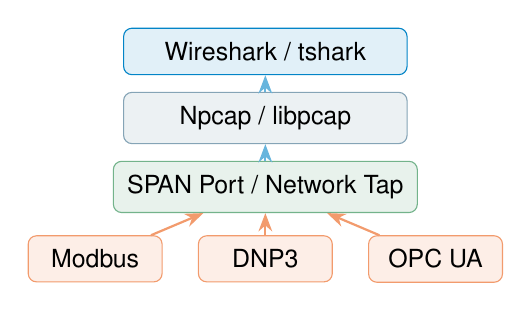
\begin{tikzpicture}[
  blk/.style={rectangle, rounded corners=3pt, draw, fill, text centered,
    font=\small\sffamily, inner sep=5pt, minimum width=3.6cm, minimum height=0.58cm},
  arr/.style={-Stealth, thick}
]
\node[blk, draw=wblue, fill=wblue!12] (ws) {Wireshark / tshark};
\node[blk, draw=wnavy!50, fill=wnavy!8, below=6pt of ws] (npcap) {Npcap / libpcap};
\node[blk, draw=wgreen!60, fill=wgreen!10, below=6pt of npcap] (span) {SPAN Port / Network Tap};

\node[blk, draw=worange!60, fill=worange!10, below left=8pt and -18pt of span, minimum width=1.7cm] (mb) {Modbus};
\node[blk, draw=worange!60, fill=worange!10, below=8pt of span, minimum width=1.7cm] (dnp) {DNP3};
\node[blk, draw=worange!60, fill=worange!10, below right=8pt and -18pt of span, minimum width=1.7cm] (opc) {OPC UA};

\draw[-Stealth, thick, color=wblue!60] (span) -- (npcap);
\draw[-Stealth, thick, color=wblue!60] (npcap) -- (ws);
\draw[-Stealth, thick, color=worange!60] (mb) -- (span);
\draw[-Stealth, thick, color=worange!60] (dnp) -- (span);
\draw[-Stealth, thick, color=worange!60] (opc) -- (span);
\end{tikzpicture}

\vspace{5pt}

\begin{tcolorbox}[
  enhanced, colback=waccent, colframe=wblue, arc=4pt,
  fonttitle=\small\bfseries\sffamily\color{white},
  title=Certification Relevance,
  boxed title style={colback=wblue},
  attach boxed title to top left={yshift=-2mm, xshift=5mm},
  top=8pt, bottom=6pt, left=6pt, right=6pt
]
\setlist[itemize]{noitemsep, topsep=0pt, leftmargin=*, label=\textcolor{wblue}{$\bullet$}}
\begin{itemize}\small
  \item \textbf{GICSP (GIAC)} — ICS network analysis and incident response are core exam domains; Wireshark skills are assumed.
  \item \textbf{GRID (GIAC)} — ICS defender cert; network forensics and anomaly detection heavily tested.
  \item \textbf{CEH (EC-Council)} — Packet analysis and protocol investigation in network recon modules.
  \item \textbf{CompTIA CySA+} — Network traffic analysis in the threat detection domain.
\end{itemize}
\end{tcolorbox}

\vspace{5pt}

\begin{tcolorbox}[
  enhanced, colback=worange!8, colframe=worange, arc=4pt,
  fonttitle=\small\bfseries\sffamily\color{white},
  title=Next Steps (Certs),
  boxed title style={colback=worange},
  attach boxed title to top left={yshift=-2mm, xshift=5mm},
  top=8pt, bottom=6pt, left=6pt, right=6pt
]
\begin{enumerate}[noitemsep, topsep=0pt, leftmargin=*, label=\small\textcolor{worange}{\arabic*.}]
  \item \small Complete Wireshark as the final course in the 8-guide sequence.
  \item Configure a home lab tap or SPAN port and capture live protocol traffic.
  \item Register at \texttt{giac.org} for GICSP; review the exam objectives and map to completed courses.
  \item GICSP requires no specific experience; exam available at Pearson VUE centers.
\end{enumerate}
\end{tcolorbox}

\vspace{3pt}

\begin{center}
\begin{tikzpicture}
  \foreach \val/\lbl/\col [count=\i] in {
    10/Chapters/wblue,
    400+/Questions/worange,
    Free/Tool/wgreen
  }{
    \node[rectangle, rounded corners=3pt, fill=\col!12, draw=\col!40,
          inner sep=5pt, minimum width=1.1cm, font=\sffamily, text=\col] at (\i*1.35, 0)
      {\textbf{\val}\\\tiny\\color{\1}\lbl};
  }
\end{tikzpicture}
\end{center}

\end{minipage}

\begin{tikzpicture}[remember picture, overlay]
  \fill[wnavy!90] (current page.south west) rectangle ([yshift=0.32in]current page.south east);
  \node[anchor=west, text=white!70, font=\footnotesize\sffamily]
    at ([xshift=0.65in, yshift=0.16in]current page.south west)
    {SCADA Hub Training Platform · scada-hub.vercel.app · Free access · No account required for study material};
  \node[anchor=east, text=wcyan, font=\footnotesize\bfseries\sffamily]
    at ([xshift=-0.65in, yshift=0.16in]current page.south east)
    {Course 8 of 8};
\end{tikzpicture}

\end{document}
